\documentclass{article}  % list options between brackets
\usepackage{bmpsize}
\usepackage[dvipdfmx]{graphicx}              % list packages between braces
\usepackage{url}
\usepackage{color}
\usepackage{amsmath}
\usepackage{amsfonts}
\usepackage{hyperref}
\usepackage{epstopdf}

\begin{document}
\title{Notes on Support Vector Machine}
\author{greeness}
%\date{}                                           % Activate to display a given date or no date


\maketitle

\section{Notation}

We use $y\in\{-1,1\}$ to denote the class labels. We use parameters $w,b$ and write out classifier as 
$g(w^Tx+b)$, where $b$ is the intercept term (or bias).  From our definition of $g$, our classifier will directly predict either 1 or -1 ~\cite{ng-lecture}.

\section{Functional Margin}

Given a training example ($x^{(i)}, y^{(i)}$), we define the function margin of ($w,b$) with respect to the training example
\[
\hat \gamma ^{(i)} = y^{(i)}(w^Tx + b).
\]
Note that if $y{(i)}$ = 1, then for the functional margin to be large, we need $w^Tx+b$ to be a large positive number. Conversely, if $y{(i)}$ = -1, then for the functional margin to be large, we need $w^Tx+b$ to be a large negative number. 

Given a training set $S = \{ \}$, we define the function margin of ($w,b$) with respect to $S$ to be the smallest of the functional margins of the individual training examples. 
\[
\hat \gamma = \min_{i=1,\cdots, m} \hat \gamma ^{(i)}.
\]

\section{Geometric Margin}
First since the decision boundary is defined by $w^Tx+b=0$, we immediately know that $w$ is orthogonal (at 90$^\circ$) to the separating hyperplane. 

\begin{figure}[htbp]
   \centering
   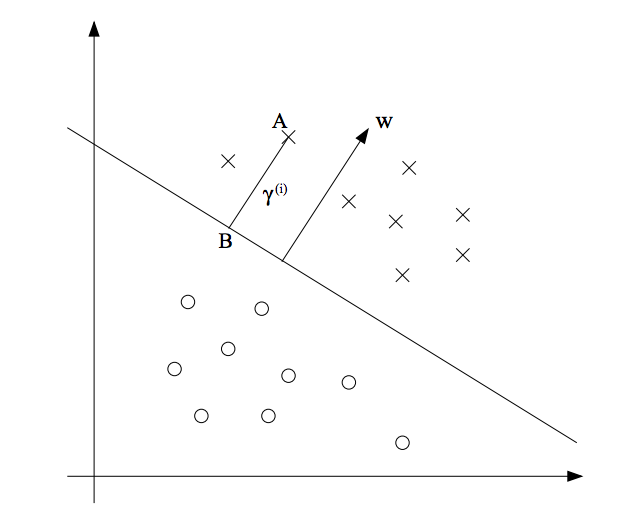
\includegraphics[scale=0.7]{geometric_margin.png} 
   \caption{Geometric Margin example}
   \label{fig:geometric_margin_example}
\end{figure}

Consider the point at $A$, which represents the input $x^{(i)}$ of some training example with label $y^{(i)} = 1$. Its distance to the decision boundary, $\gamma ^{(i)}$, is given by the line segment $AB$. 

\begin{itemize}
\item $w/||w||$ is a unit-length vector pointing in the same direction as $w$;
\item $A$ represent $x^{(i)}$, $\overrightarrow{A} = x^{(i)}$
\item $\overrightarrow{BA} = \gamma ^ {(i)} \frac{w}{||w||}$ (Think about vector length $\times$ vector direction)
\item Consider $\overrightarrow{A} = \overrightarrow{B} + \overrightarrow{BA}$
\item we therefore find that the point $\overrightarrow{B} = \overrightarrow{A} - \overrightarrow{BA} = x^{(i)} - \gamma^{(i)} \cdot \frac{w}{||w||}.$
\end{itemize}

Considering point $B$ lies on the decision boundary and all points $x$ on the decision boundary satisfy the equation $w^Tx+b = 0$. 
\[ w^T\left( x^{(i)} - \gamma^{(i)} \cdot \frac{w}{||w||}\right) + b= 0.
\]
Solving for $\gamma^{(i)}$ yields 
\[
\gamma^{(i)} = \frac{w^Tx^{(i)}+b}{||w||} = \left(\frac{w}{||w||}\right)^T x^{(i)} + \frac{b}{||w||}.
\]
The above is  a solution for the case of a positive training example at $A$ in the figure. More generally, we define the geometric margin of $(w,b)$ with respect to a training example ($x^{(i)}, y^{(i)}$) to be
\[
\gamma^{(i)} = y^{(i)} \left[\left(\frac{w}{||w||}\right)^T x^{(i)} + \frac{b}{||w||} \right].
\]

Not that if $||w||=1$, then the functional margin equals the geometric margin. Also the geometric margin is invariant to rescaling of the parameters.  

Given a training set $S = \{ \}$, we define the geometric margin of ($w,b$) with respect to $S$ to be the smallest of the geometric margins of the individual training examples. 
\[
\gamma = \min_{i=1,\cdots, m}\gamma ^{(i)}.
\]


\begin{thebibliography}{9}

\bibitem{ng-lecture} Anrew Ng, \emph{CS229 Lecture notes - Support Vector Machine}, \url{http://cs229.stanford.edu/notes/cs229-notes3.pdf}.

\end{thebibliography}


\end{document}  